\subsection{Morphology and Filtering}

The Morphology and Filtering component of the algorithm takes the foreground mask as input from the background subtractor removing noise and combining foreground objects together that are fractured. 

\subsubsection{Median Filtering}

Often salt and pepper noise is generated by the subtraction process due to lighting changes, camera instability and non-target object movement like trees and humans. By applying a median filter (\ref{subsubsection:median_filter}) this noise can be removed. Figure \ref{fig:mask_saltnpepper} shows the effect of applying a median filter to remove noise from a foreground mask. It's important to remove this noise because it's doesn't represent a vehicle and it may lead to incorrect data collection output. The OpenCV method medianBlur() was used to implement this functionality.

\subsubsection{Morphology}

Vehicles sometimes do not form a connected-component of 1-pixels in the foreground mask. The GMM clusters pixels on their colour so any parts of a vehicle that appear similar in colour to the background distribution, which is most often the colour of the road, are classified as background pixels. Car windows in particular are incorrectly classified as background pixels because they reflect light from the road. This phenomenon can cause a single vehicle to be represented in the foreground mask as a number of disconnect-components. This is bad as it appears to other parts of the algorithm that there are more vehicles than one. Figure \ref{fig:example_subtraction} shows an example of a single vehicle generating many distinct blobs. By applying morphology to the foreground mask these blobs can be recombined into a single entity.

To recombine fractured blobs a morphological closing and dilation (\ref{subsubsection:morphology}) are performed, Figure \ref{fig:morphed} shows an example of blob recombination. The OpenCV function morphologyEx() was used to perform these operations. The selection of structuring element shapes, size and number of iterations is dependent on the specific traffic scene presented and requires considerable calibration. 

\subsubsection{Calibration}

Usually at least one region of the foreground mask has more correct pixel clustering than another, this is often a consequence of the lighting in that region of the input images. When calibrating the morphological operations the area to focus on improving is this region. In a situations where the camera perspective is not directly above the traffic setting looking down it's not possible to improve all regions of the image as the perceived size of the vehicles changes throughout the image. Hence, the morphological structuring should be selected for a specific region of improvement. In situations where the camera perspective is perpendicular to vehicle movement, the structuring element selection will work for the entire image as vehicle scale doesn't change. Figure \ref{fig:perspective} illustrates the difference in these perspectives.

\begin{figure}[h]
    \centering
     \begin{subfigure}[b]{0.45\textwidth}
        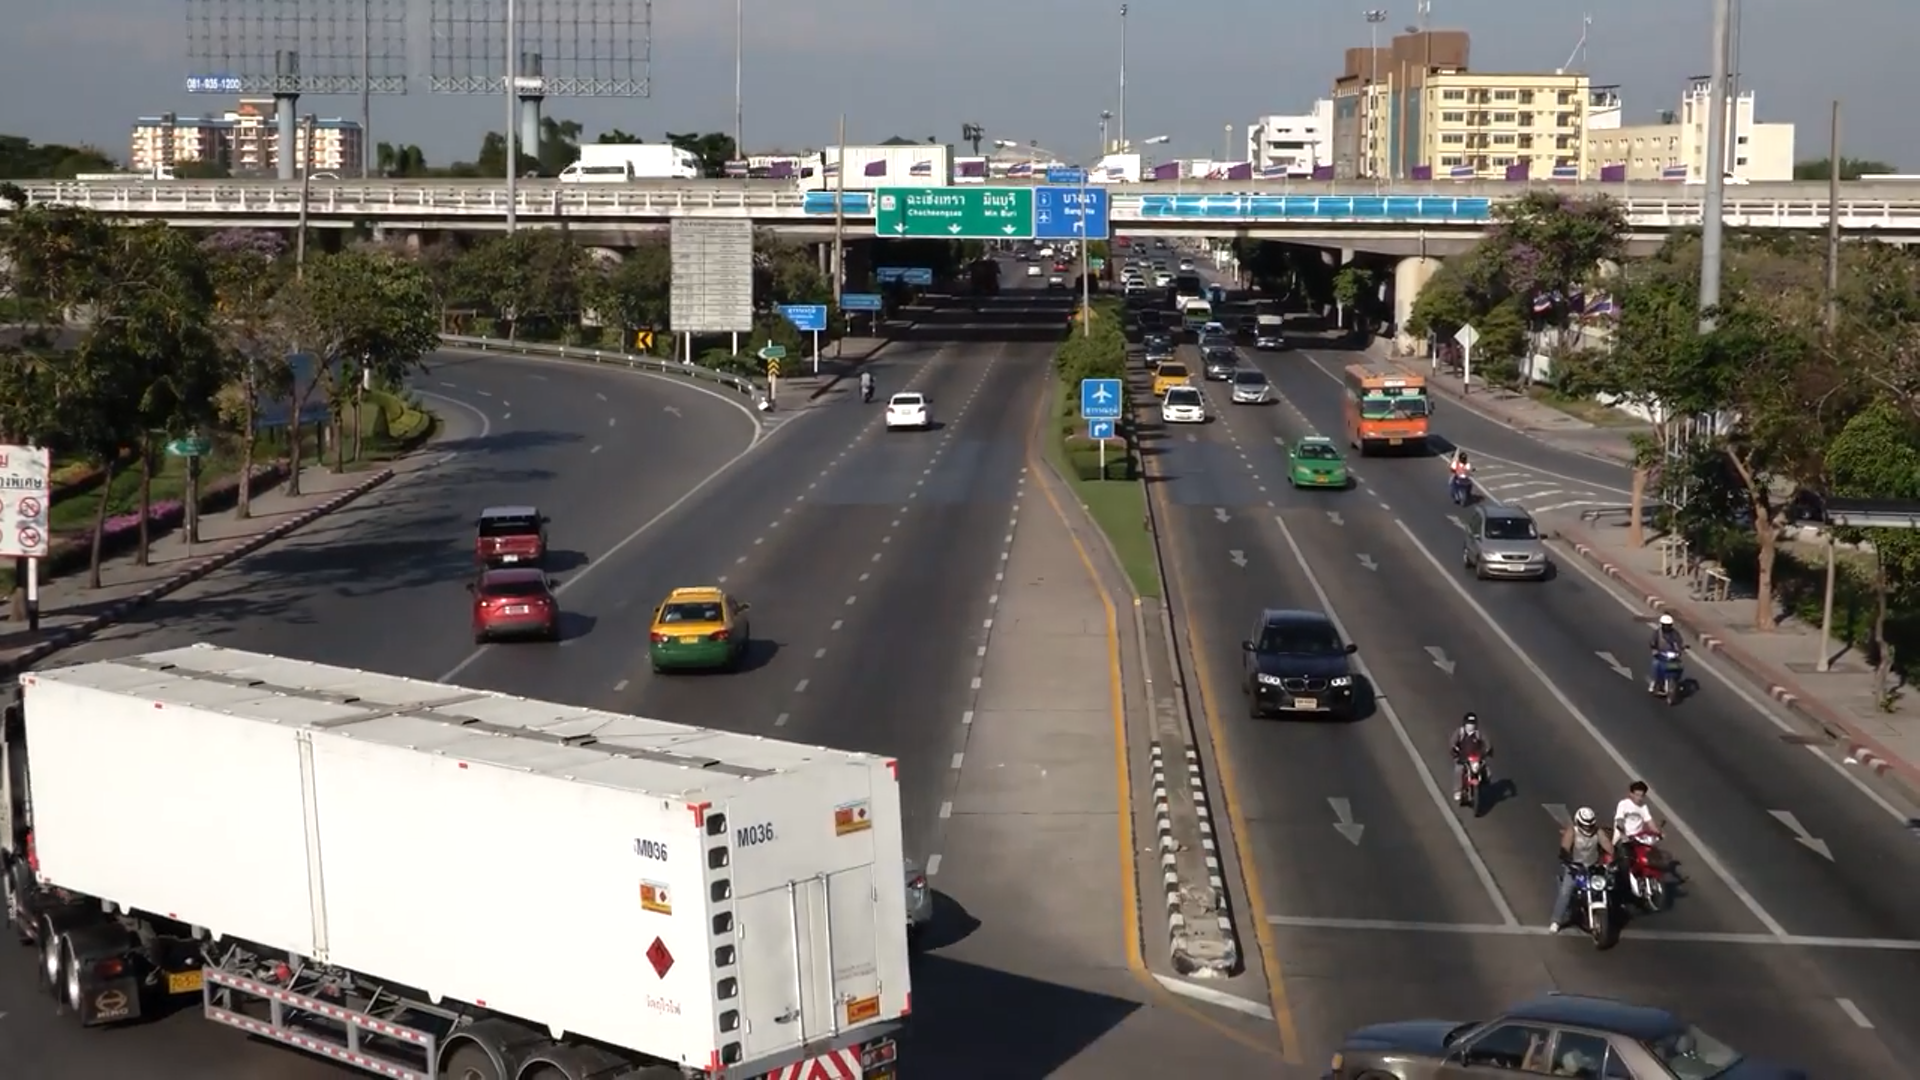
\includegraphics[width=\textwidth]{design/detection/morphology/perspectiveA}
	\captionsetup{format = hang}
        \caption{Changing vehicle scale perspective.}
    \end{subfigure} 
    \begin{subfigure}[b]{0.45\textwidth}
        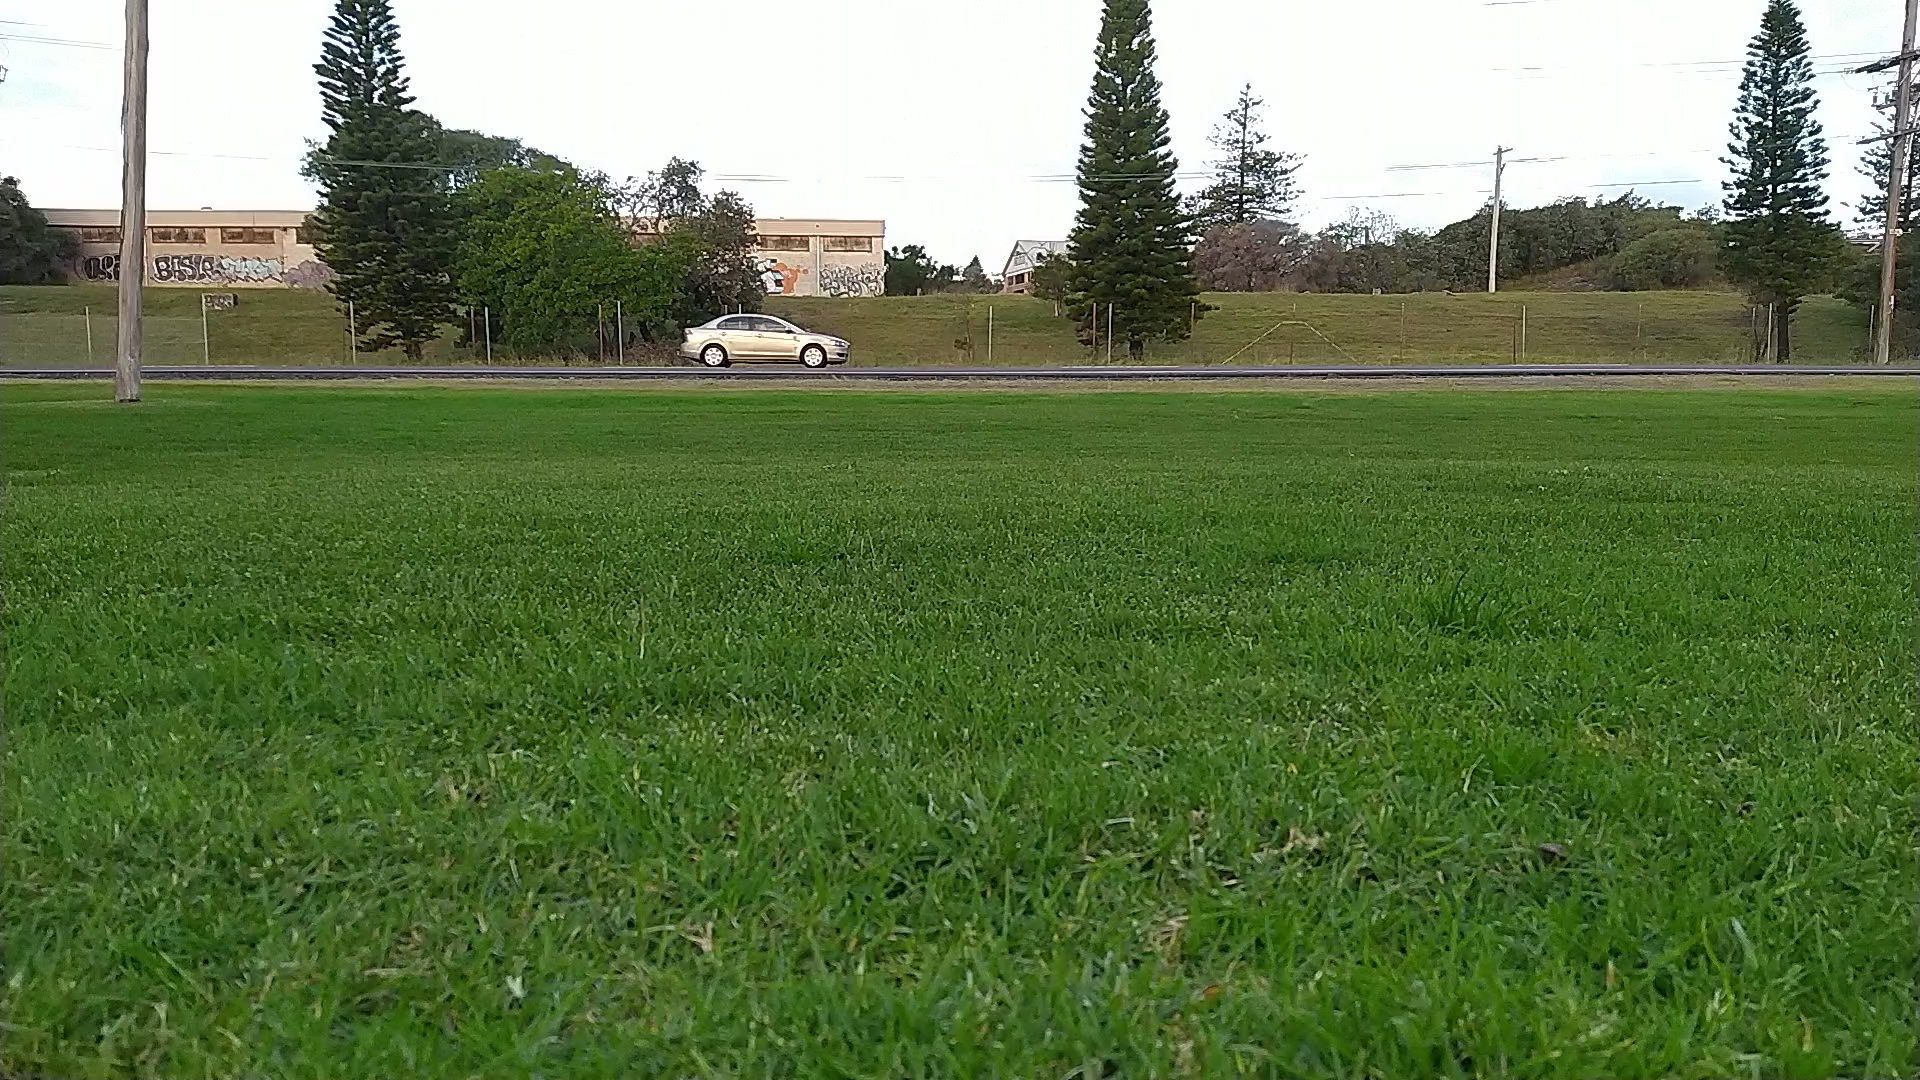
\includegraphics[width=\textwidth]{design/detection/morphology/perspectiveB}	
	\captionsetup{format = hang}
        \caption{Fixed vehicle scale perspective.}
    \end{subfigure}
    \captionsetup{format = hang}
    \caption{Comparison of camera perspective and its affect on vehicle scale.}
    \label{fig:perspective}
\end{figure}

Morphological operations can be computationally expensive depending on the size of the structuring element and number of iterations performed. In order to maintain real-time image processing minimising these factors for each traffic scenario is important. Figure \ref{fig:morph_testing} shows the comparative performance of three structuring element shapes on the same foreground mask for a 7x7 element size and varying iterations. Visual analysis of each outcome showed that the rectangular element performed for 3 iterations gave the best result because it generated the best recombination of blobs. Figure \ref{fig:compare_closure} shows an example blob recombination, in this case the rectangular structuring element successfully recombined the blob where the elliptical element could not.

\begin{figure}[H]
    \centering
    \begin{subfigure}[b]{0.45\textwidth}
        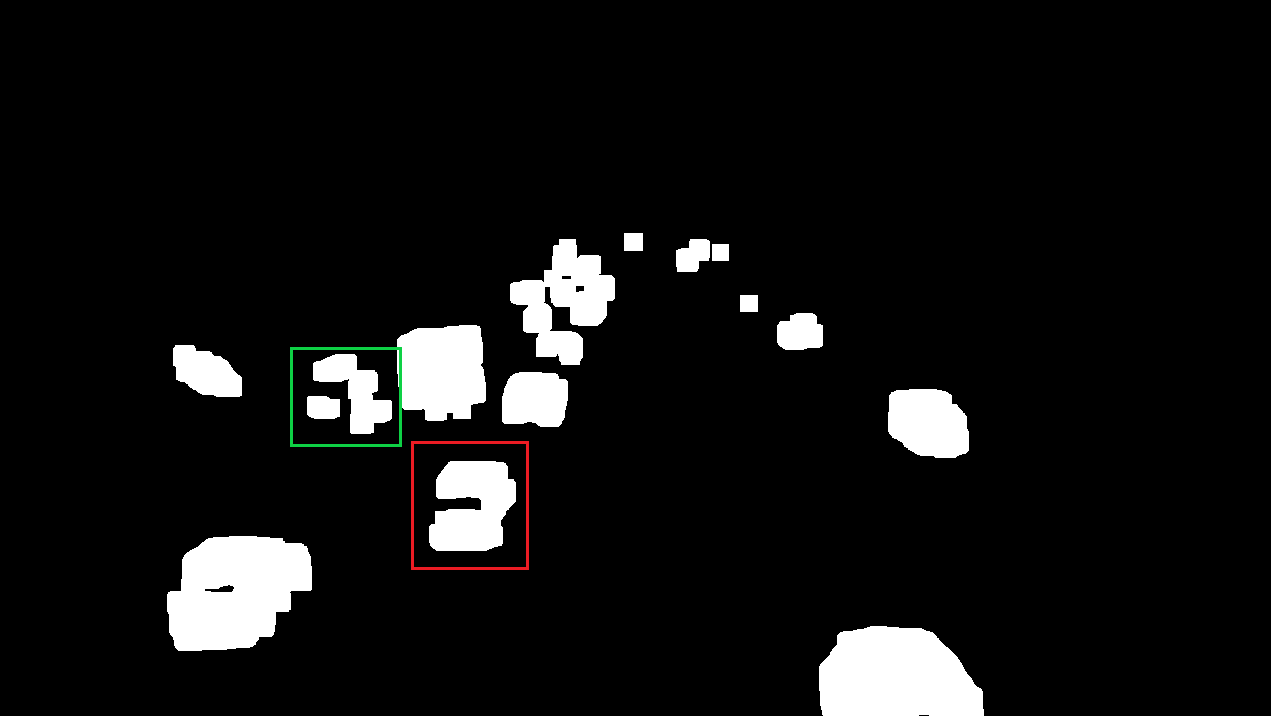
\includegraphics[width=\textwidth]{design/detection/calibration/rect_3_edit}
        \caption{Closure with rectangle.}
    \end{subfigure}
    \begin{subfigure}[b]{0.45\textwidth}
        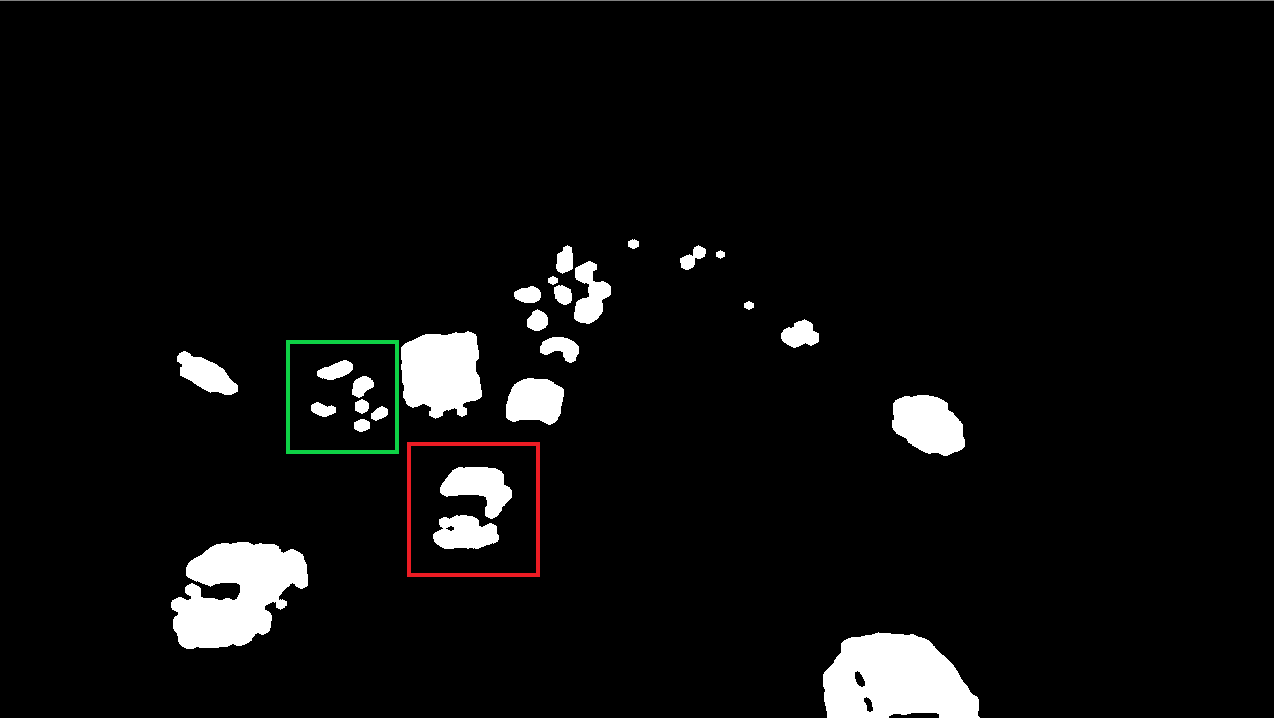
\includegraphics[width=\textwidth]{design/detection/calibration/ellipse_3_edit}
        \caption{Closure with ellipse.}
    \end{subfigure}
    \captionsetup{format = hang}
    \caption{Comparison of morphological closure using a 7x7 rectangular and elliptical structuring element for 3 iterations.}
    \label{fig:compare_closure}
\end{figure}


\begin{figure}[H]
    \begin{tabular}{
        >{\centering\arraybackslash}m{0.4cm}
        >{\centering\arraybackslash}m{4.5cm}
        >{\centering\arraybackslash}m{4.5cm}
        >{\centering\arraybackslash}m{4.5cm}}
          & Ellipse & Cross & Rectangle \\
        1 
        &
        \begin{subfigure}[b]{0.3\textwidth}
            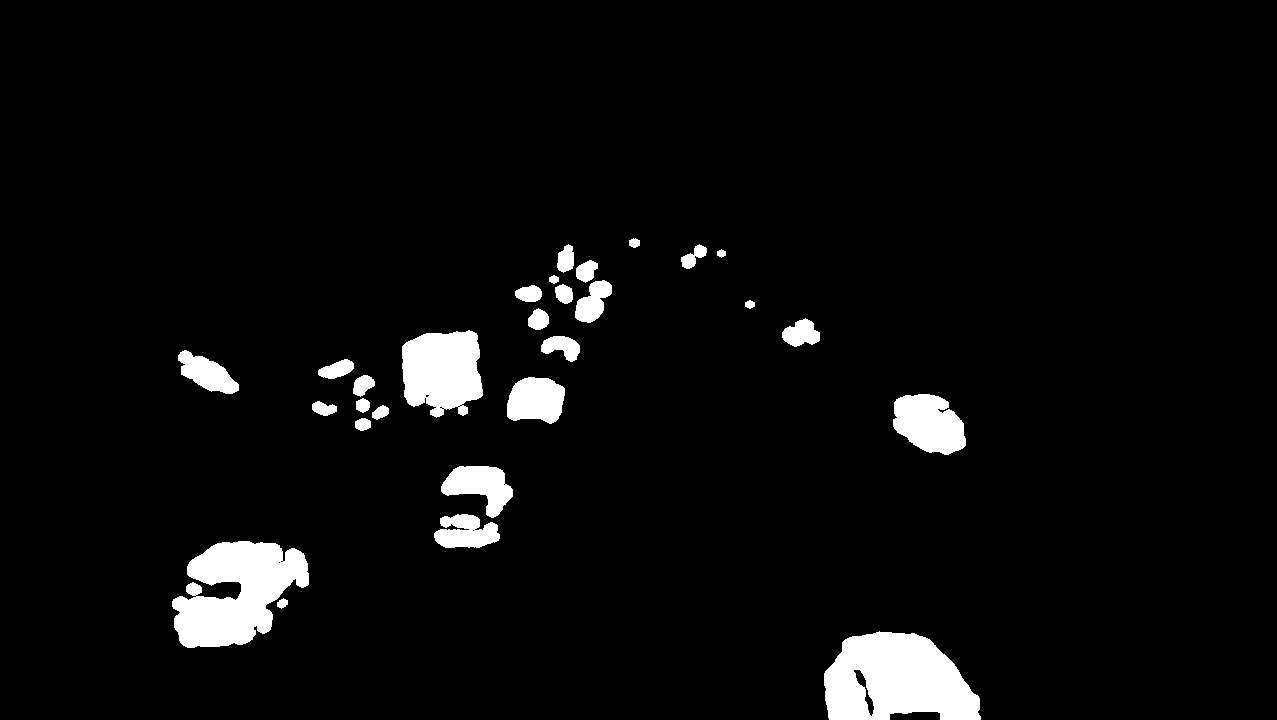
\includegraphics[width=\textwidth]{design/detection/morphology/ellipse_1}
            % \captionsetup{format = hang}
        \end{subfigure} &
        \begin{subfigure}[b]{0.3\textwidth}
            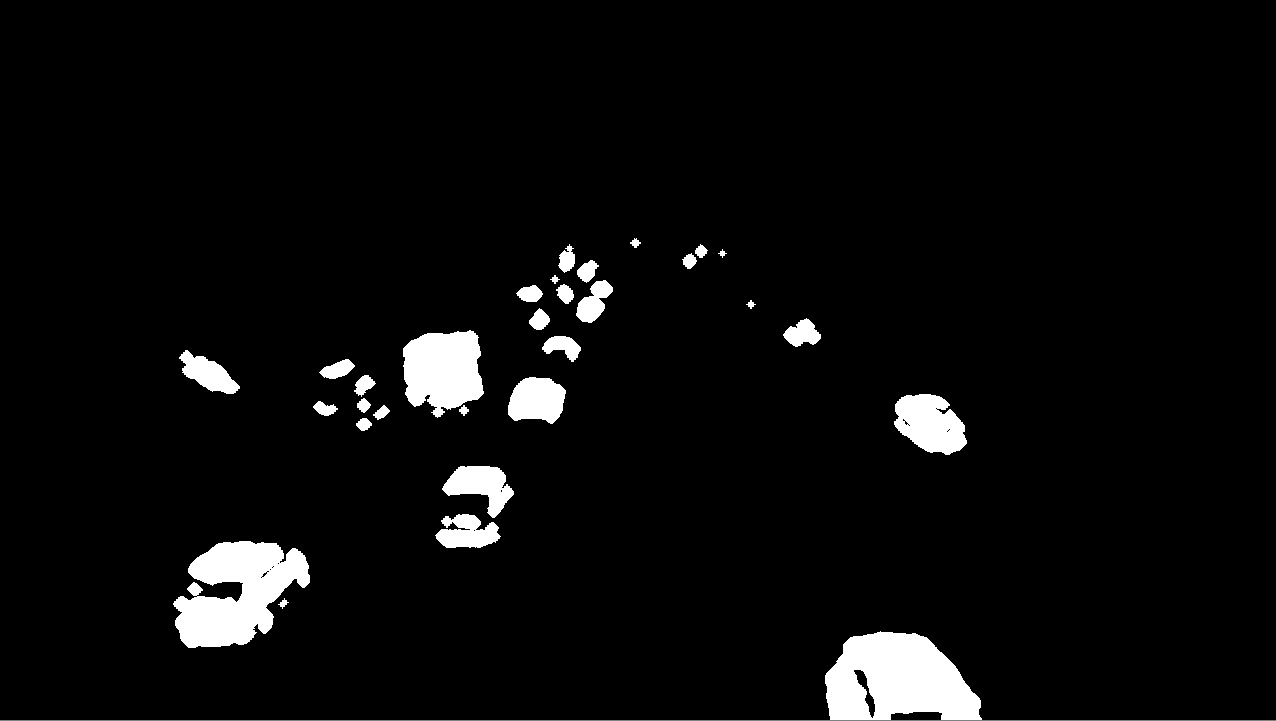
\includegraphics[width=\textwidth]{design/detection/morphology/cross_1}
            % \captionsetup{format = hang}
        \end{subfigure} &
        \begin{subfigure}[b]{0.3\textwidth}
            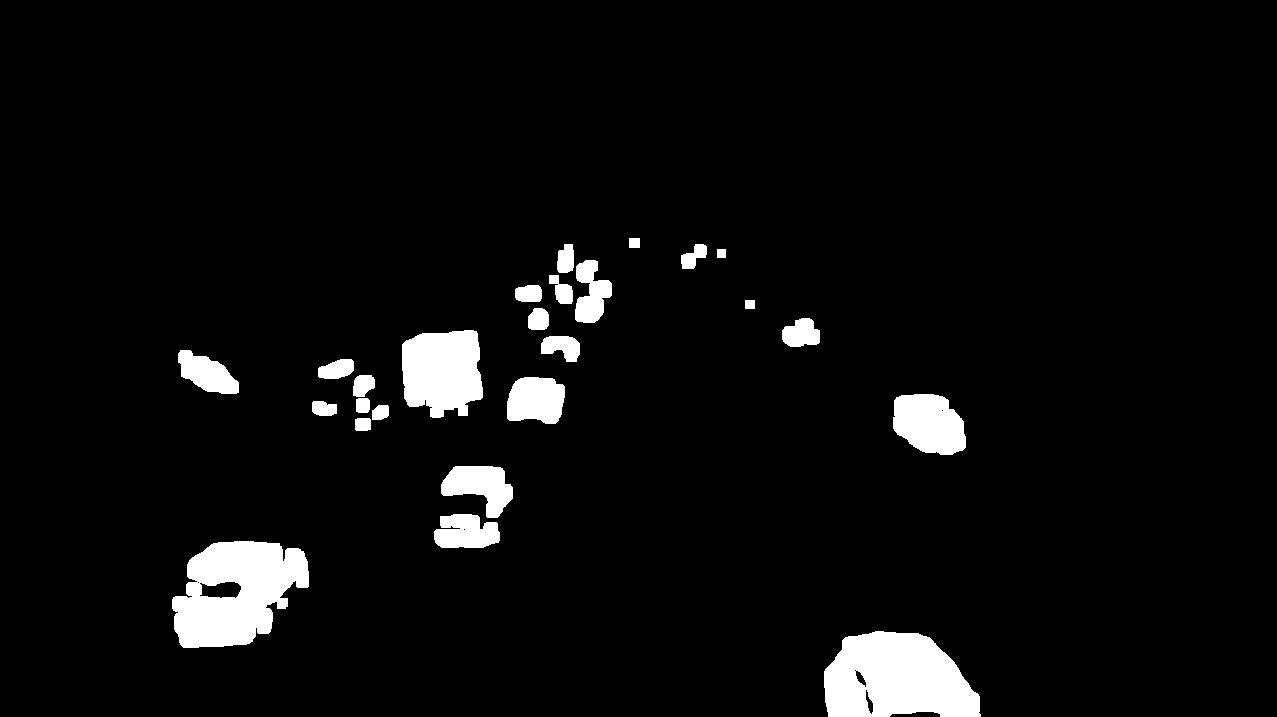
\includegraphics[width=\textwidth]{design/detection/morphology/rect_1}
            % \captionsetup{format = hang}
        \end{subfigure} \\
        3 &
        \begin{subfigure}[b]{0.3\textwidth}
            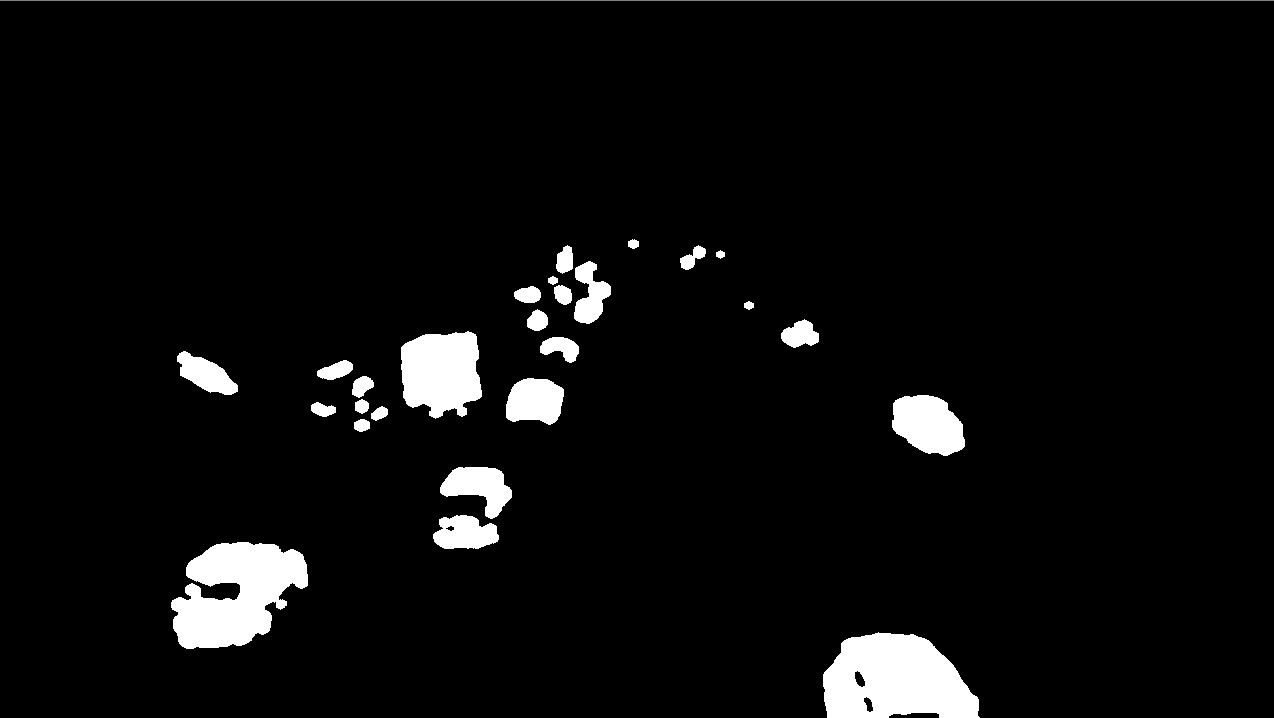
\includegraphics[width=\textwidth]{design/detection/morphology/ellipse_3}
            % \captionsetup{format = hang}
        \end{subfigure} &
        \begin{subfigure}[b]{0.3\textwidth}
            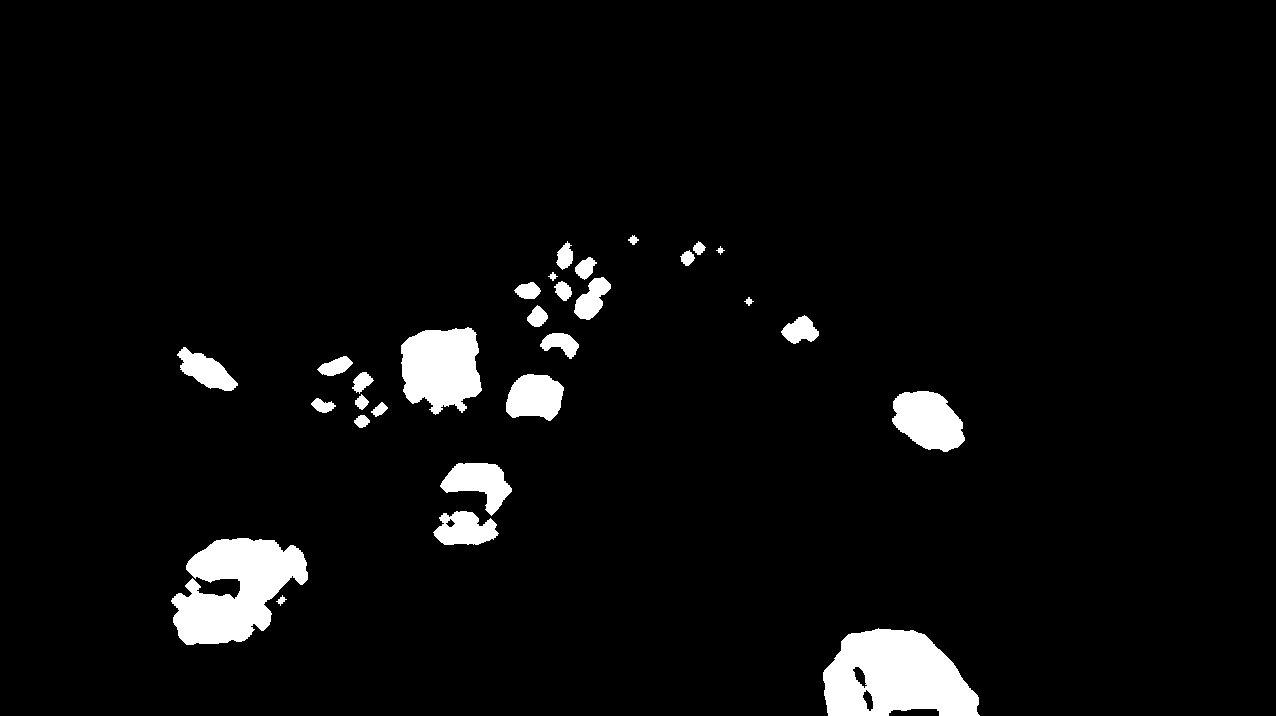
\includegraphics[width=\textwidth]{design/detection/morphology/cross_3}
            % \captionsetup{format = hang}
        \end{subfigure} &
        \begin{subfigure}[b]{0.3\textwidth}
            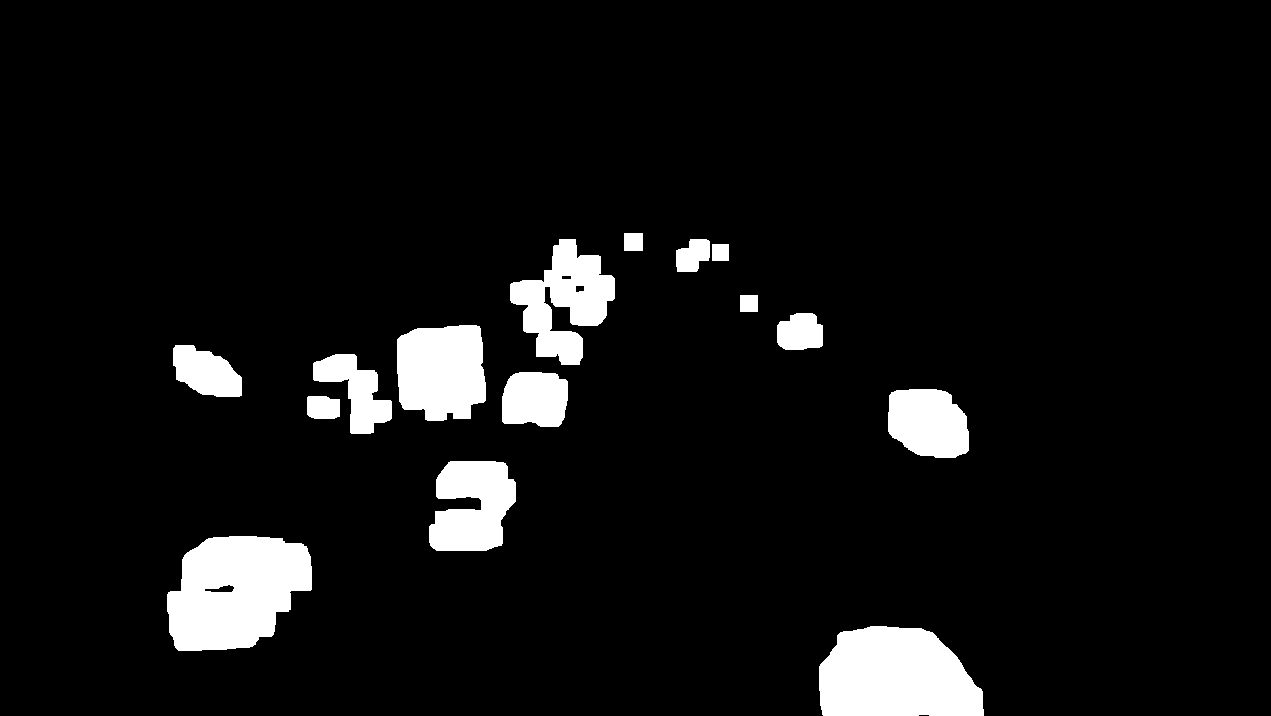
\includegraphics[width=\textwidth]{design/detection/morphology/rect_3}
            % \captionsetup{format = hang}
        \end{subfigure} \\
        5 &
        \begin{subfigure}[b]{0.3\textwidth}
            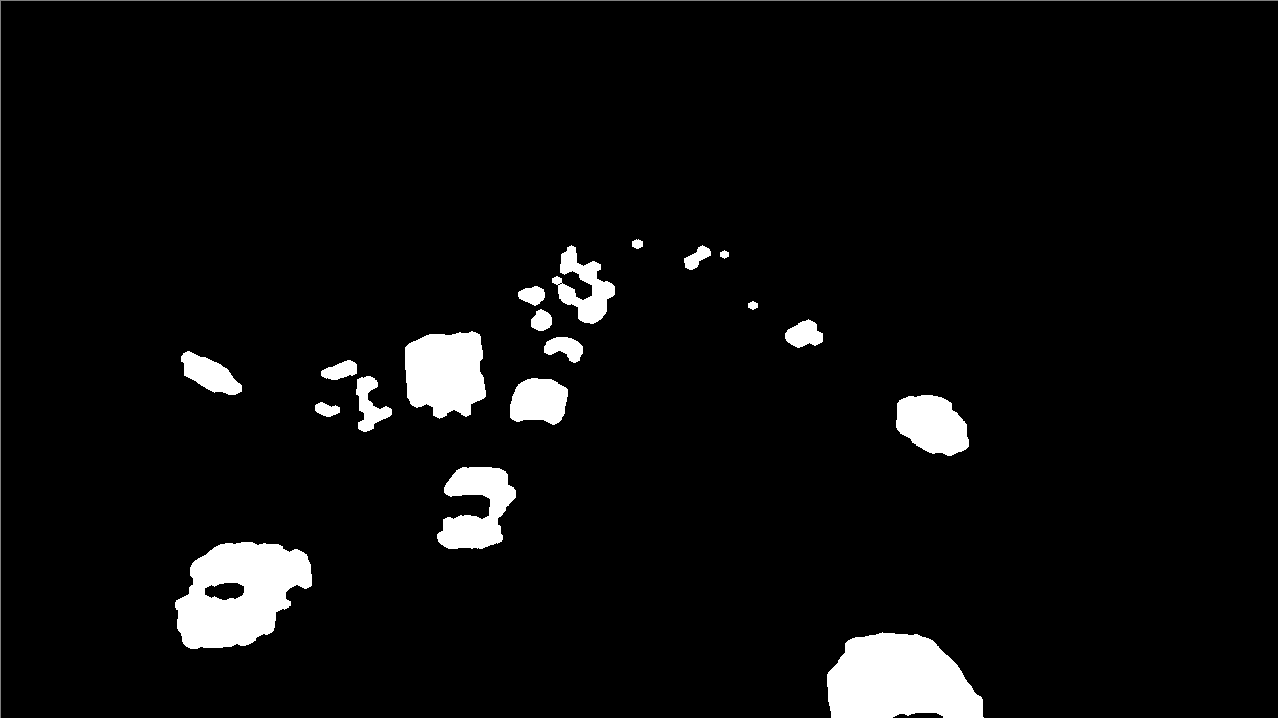
\includegraphics[width=\textwidth]{design/detection/morphology/ellipse_5}
            % \captionsetup{format = hang}
        \end{subfigure} &
        \begin{subfigure}[b]{0.3\textwidth}
            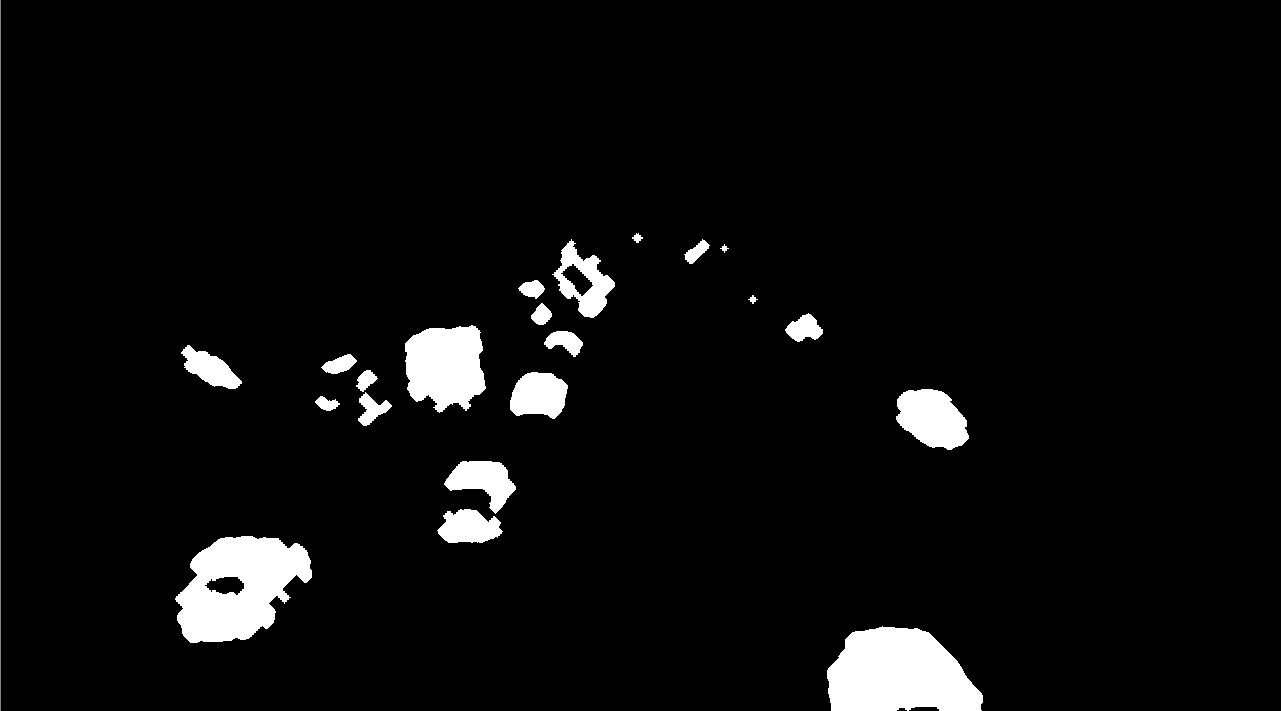
\includegraphics[width=\textwidth]{design/detection/morphology/cross_5}
            % \captionsetup{format = hang}
        \end{subfigure} &
        \begin{subfigure}[b]{0.3\textwidth}
            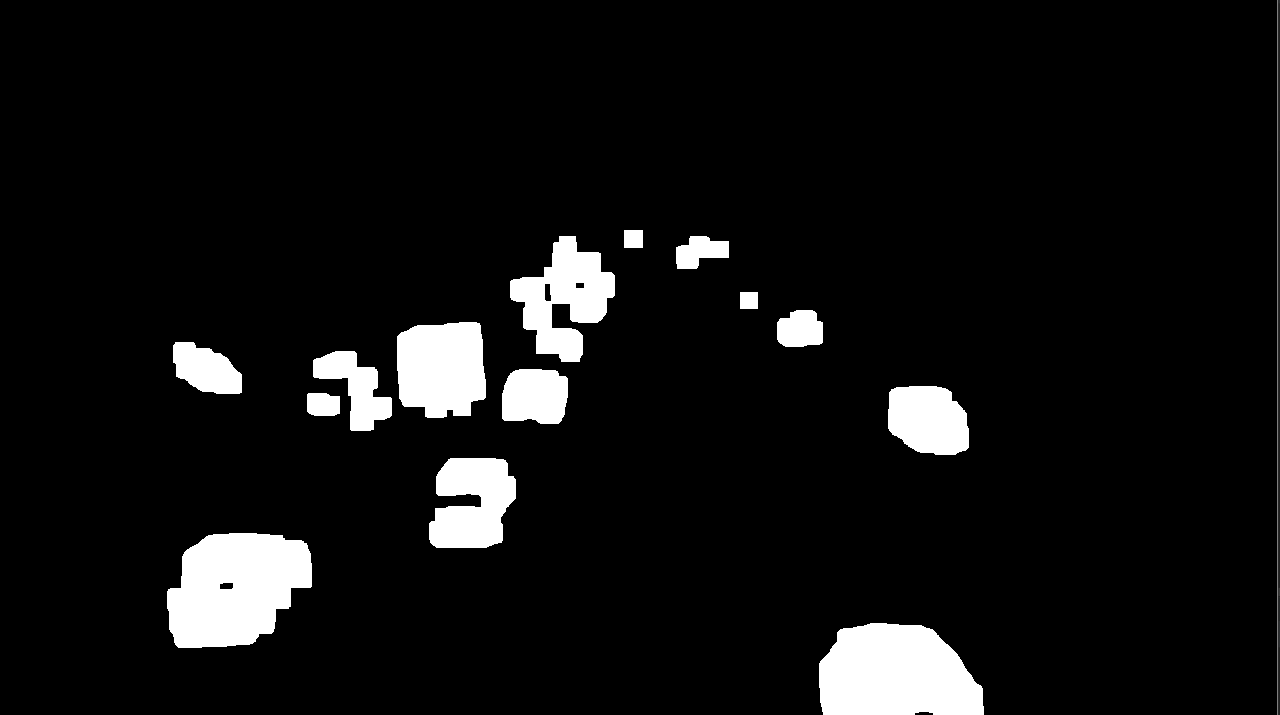
\includegraphics[width=\textwidth]{design/detection/morphology/rect_5}
            % \captionsetup{format = hang}
        \end{subfigure} \\
    \end{tabular}
    \captionsetup{format = hang}
    \caption{Morphological closing using different 7x7 structuring elements and iterations.}
    \label{fig:morph_testing}
\end{figure}
